\subsection{FINITE COXETER GROUPS}

In this section, we are going to determine, up to isomorphism, all root systems, and consequently all crystallographic groups (§ 2, no. 5). More generally, we shall start by determining all finite groups generated by reflections in a finite-dimensional real vector space: this is equivalent (Chap. V. § 4, no. 8) to determining all finite Coxeter groups, or (Chap. V. § 4, no. 8, Th. 2) to determining all Coxeter matrices of finite order such that the associated bilinear form is positive and non-degenerate.

Let \(\mathrm{M} = (m_{ij})_{i,j\in \mathbb{I}}\) be a Coxeter matrix of finite order \(l\) . Put

\[
q _ {i j} = - \cos (\pi / m _ {i j}).
\]

Recall that \(q_{ii} = 1\) and that \(q_{ij} = q_{ji}\) is zero or \(\leqslant -1/2\) for \(i \neq j\) . Put \(E = R^l\) and let \((c_i)_{i \in I}\) be the canonical basis of \(E\) . Denote by \((x|y)\) the bilinear form on \(E\) associated to \(M\) (Chap. V, § 4. no. 1) and \(q\) the quadratic form \(x \mapsto (x|x)\) on \(E\) . For \(x = \sum_{i \in I} \xi_i x_i\) ,

\[
\| x \| ^ {2} = q (x) = \sum_ {i, j \in I} q _ {i j} \xi_ {i} \xi_ {j}.
\]

Denote by (X, f) the Coxeter graph of M (Chap. IV, § 1, no. 9). If \(a\) is an edge of X, \(f(a)\) is called the order of \(a\) .

In the remainder of this number, the Coxeter group \(W(M)\) defined by M (Chap. V, § 4, no. 3) is assumed to be finite, so that q is positive and non-degenerate and X is a forest (Chap. V, § 4, no. 8, Prop. 8). We also assume that X is connected (in other words that the Coxeter group \(W(M)\) is irreducible), so that X is a tree.

From the condition that q is positive and non-degenerate, we shall obtain conditions on the \(m_{ij}\) that will enable us to list all the possibilities for the corresponding Coxeter graphs; it will only remain to show that these possibilities are actually realised, in other words that the corresponding groups W(M) are finite.

Lemma 1. For all \(i\) , \(\sum_{j \neq i} q_{ij}^2 < 1\) .

Let \(J\) be the set of \(j \in I\) such that \(q_{ij} \neq 0\) , in other words such that \(\{i, j\}\) is an edge of \(X\) . If \(j, j' \in J\) and \(j \neq j'\) , \(\{j, j'\}\) is not an edge (otherwise \(i, j, j'\) would form a circuit), so \((e_j | e_{j'}) = 0\) . Let \(F = \sum_{j \in J} R e_j\) . Then \((e_j)_{j \in J}\) is an orthonormal basis of \(F\) . The distance \(d\) from \(e_i\) to \(F\) is given by \(d^2 = 1 - \sum_{j \in J} (e_i | e_j)^2 = 1 - \sum_{j \in J} q_{ij}^2 = 1 - \sum_{j \neq i} q_{ij}^2\) , hence the lemma.

Indeed, if i is linked to h other vertices, the relations \(q_{ij}^{2} \geqslant \frac{1}{4}\) for these other vertices implies that \(\frac{h}{4} < 1\) by Lemma 1, so \(h \leqslant 3\) .

Lemma 3. If \(i\) belongs to 3 edges, these edges are of order 3.

If not, we would have, in view of the relation \(\cos \frac{\pi}{4} = \frac{\sqrt{2}}{2}\) ,

\[
\sum_ {j \neq i} q _ {i j} ^ {2} \geqslant \frac {1}{4} + \frac {1}{4} + (\frac {\sqrt {2}}{2}) ^ {2} = 1
\]

which is impossible (Lemma 1).

Lemma 4. If there exists an edge of order \(\geqslant 6\) , then \(l = 2\) .

Indeed, let \(\{i,j\}\) be such an edge. If l \textgreater{} 2, one of the edges i, j (say i) would be linked to a third vertex \(j'\) , since X is connected. In view of the relation \(\cos \frac{\pi}{6} = \frac{\sqrt{3}}{2}\) we would have

\[
\sum_ {k \neq i} q _ {i k} ^ {2} \geqslant \frac {1}{4} + (\frac {\sqrt {3}}{2}) ^ {2} = 1
\]

which is impossible (Lemma 1).

Lemma 5. A vertex cannot belong to two distinct edges of order \(\geqslant 4\) .

Let \(i\) be such a vertex. We would have \(\sum_{j\neq i}q_{ij}^{2}\geqslant (\frac{\sqrt{2}}{2})^{2} + (\frac{\sqrt{2}}{2})^{2} = 1\) , which is impossible (Lemma 1).

Let \(\{i, j\}\) be an edge of \(X\) . We are going to define a new Coxeter graph, which will be obtained from the graph of \(M\) by identifying \(i\) and \(j\) . The set \(I'\) of its vertices is the quotient of \(I\) obtained by identifying \(i\) and \(j\) . Put \(p = \{i, j\}\) , which is an element of \(I'\) , and identify the elements of \(I\) distinct from \(i\) and \(j\) with their canonical images in \(I'\) . Let \(k, k'\) be two distinct elements of \(I'\) . Then, \(\{k, k'\}\) is an edge of the new graph in the following cases:

\begin{enumerate}
\def\labelenumi{\arabic{enumi})}
\item
  \(k\) and \(k'\) are distinct from \(p\) and \(\{k, k'\}\) is an edge of \(X\) : in this case, the order of this edge is defined to be \(m_{kk'}\) :
\item
  \(k = p\) , and one of the sets \(\{i, k'\}, \{j, k'\}\) is an edge of \(X\) ; the order of \(\{p, k'\}\) is defined to be \(m_{ik'}\) if \(\{i, k'\}\) is an edge of \(X\) , and \(m_{jk'}\) if \(\{j, k'\}\) is an edge of \(X\) (these two possibilities are mutually exclusive because \(X\) is a tree).
\end{enumerate}

Let \(M' = (m_{ij}')_{i,j \in I'}\) be the new Coxeter matrix thus defined, and put \(q_{ij}' = -\cos \frac{\pi}{m_{ij}'}\) . Then, for \(k \neq p\) , \(l_{pk}' = q_{ik} + q_{jk}\) . Thus, if \((\xi_i) \in \mathbf{R}^{I'}\) ,

\[
\begin{array}{r l} \sum_ {k, k ^ {\prime} \in I ^ {\prime}} q _ {k k ^ {\prime}} ^ {\prime} \xi_ {k} \xi_ {k ^ {\prime}} & = \sum_ {k, k ^ {\prime} \in I} q _ {k k ^ {\prime}} \xi _ {k} \xi_ {k ^ {\prime}} + \xi_ {p} ^ {2} - \xi_ {i} ^ {2} - \xi_ {j} ^ {2} - 2 q _ {i j} \xi_ {i} \xi_ {j} \\ & = \sum_ {k, k ^ {\prime} \in I} q _ {k k ^ {\prime}} \xi _ {k} \xi_ {k ^ {\prime}} - (1 + 2 q _ {i j}) \xi_ {p} ^ {2}. \end{array} \tag {1}
\]

Lemma 6. If \(\{i,j\}\) is of order 3. \(\mathbf{W}(\mathbf{M}')\) is a finite Coxeter group.

Indeed, \(q_{ij} = -\frac{1}{2}\) , so (1) becomes

\[
\sum_ {k, k ^ {\prime} \in I ^ {\prime}} q _ {k, k ^ {\prime}} ^ {\prime} \xi_ {k} \xi_ {k ^ {\prime}} = \sum_ {k, k ^ {\prime} \in I} q _ {k, k ^ {\prime}} \xi_ {k} \xi_ {k ^ {\prime}}
\]

and \((\xi_k)_{k\in I'}\mapsto \sum_{k,k'\in I'}q_{k,k'}'\xi_k\xi_{k'}\) is a positive non-degenerate quadratic form. It now suffices to apply Th. 2 of Chap. V. § 4, no. 8.

Lemma 7. We have one of the following:

\begin{enumerate}
\def\labelenumi{\alph{enumi})}
\item
  X has a unique ramification point (Chap. IV, Appendix, no. 1), and all the edges of X are of order 3.
\item
  X is a chain and has at most one edge of order \(\geqslant 4\) .
\end{enumerate}

We argue by induction on l.

\begin{enumerate}
\def\labelenumi{\alph{enumi})}
\item
  Assume that X has a ramification point i. Then i belongs to 3 edges of order 3, \(\{i, k_{1}\}\) , \(\{i, k_{2}\}\) , \(\{i, k_{3}\}\) (Lemmas 2 and 3). If l = 4 the lemma is proved. If not, then \(k_{1}\) , say, belongs to an edge distinct from those just mentioned since X is connected. Identify i and \(k_{1}\) in the Coxeter graph of M. This gives a new graph to which the induction hypothesis can be applied, in view of Lemma 6. Now the image p of i is a ramification point of the new graph \(X'\) . Thus \(X'\) has no other ramification point and all its edges are of order 3. Thus all the edges of X are of order 3, and i and \(k_{1}\) are its only possible ramification points. But if \(k_{1}\) were a ramification point of X, p would belong to at least 4 edges in \(X'\) , contrary to Lemma 2.
\item
  Assume that X has no ramification point. Then X is a chain (Chap. IV, Appendix. no. 3, Prop. 3). Let \(\{i,j\}\) be an edge of order \(\geqslant4\) . If l=2, the lemma is trivial. If not, then i, say, belongs to an edge \(\{i,k\}\) with \(k\neq j\) (since X is connected). This edge is of order 3 (Lemma 5). Identify i and k in the Coxeter graph of M. By Lemma 6, the induction hypothesis can be applied. Let p be the image of i in the new graph \(X'\) . In \(X'\) , \(\{p,j\}\) is an edge of order \(\geqslant4\) , so \(X'\) has no other edge of order \(\geqslant4\) , and hence \(\{i,j\}\) is the only edge of order \(\geqslant4\) in X.
\end{enumerate}

Lemma 8. Let \(i_1, i_2, \ldots, i_p\) be vertices of \(X\) such that \(\{i_1, i_2\}, \{i_2, i_3\}, \ldots, \{i_{p-1}, i_p\}\) are edges of order 3. Then \(q(\sum_{r=1}^{p} re_{t_r}) = \frac{1}{2} p(p + 1)\) .

We have \((e_{i_r}|e_{i_r}) = 1, (e_{i_r}|e_{i_{r+1}}) = -\frac{1}{2}, (e_{i_r}|e_{i_s}) = 0\) if \(s > r + 1\) . Thus

\[
q \left(\sum_ {r = 1} ^ {p} r e _ {i _ {r}}\right) = \sum_ {r = 1} ^ {p} r ^ {2} - 2 \sum_ {r = 1} ^ {p - 1} \frac {1}{2} r (r + 1) = p ^ {2} - \sum_ {r = 1} ^ {p - 1} r.
\]

By Theory of Sets, Chap. III. § 5, no. 8. Cor. to Prop. 14. this is equal to

\[
p ^ {2} - \frac {1}{2} p (p - 1) = \frac {1}{2} p (p + 1).
\]

Lemma 9. Assume that X is a chain with vertices \(1,2,\ldots,l\) and edges \(\{1,2\},\{2,3\},\ldots,\{l-1,l\}\) .

\begin{enumerate}
\def\labelenumi{(\roman{enumi})}
\tightlist
\item
  If one of the edges \(\{2,3\},\{3,4\},\ldots,\{l-2,l-1\}\) is of order \(\geqslant 4\) , this edge is of order 4 and the graph is the following:
\end{enumerate}

\pandocbounded{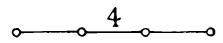
\includegraphics[keepaspectratio]{images/part002_520d8dd1.jpg}}

\begin{enumerate}
\def\labelenumi{(\roman{enumi})}
\setcounter{enumi}{1}
\tightlist
\item
  If the edge \(\{1,2\}\) is of order 5, the graph is one of the following:
\end{enumerate}

\pandocbounded{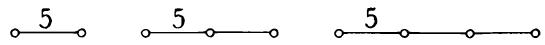
\includegraphics[keepaspectratio]{images/part002_9200390b.jpg}}

We can assume that \(l > 2\) (Lemma 4). Assume that \(\{i, i + 1\}\) is of order \(\geqslant 4\) , with \(1 \leqslant i \leqslant l - 1\) . Put

\(x = e_{1} + 2e_{2} + \dots + ie_{i}, y = e_{l} + 2e_{l - 1} + \dots + (l - i)e_{i + 1},\) and \(j = l - i\) .

By Lemma 8. \(\| x\|^2 = \frac{1}{2} i(i + 1),\| y\|^2 = \frac{1}{2} j(j + 1)\) . On the other hand, \((x|y) = ij(e_i|e_{i + 1}) = -ij\cos \frac{\pi}{m}\) with \(m = 4\) or 5 (Lemma 4). Now

\[
(x | y) ^ {2} <   \left\| x \right\| ^ {2} \| y \| ^ {2}.
\]

which gives

\[
\frac {1}{4} i j (i + 1) (j + 1) > i ^ {2} j ^ {2} \cos^ {2} \frac {\pi}{m}
\]

SO

\[
(i + 1) (j + 1) > 4 i j \cos^ {2} \frac {\pi}{m} \geqslant 2 i j.
\]

This gives, first of all, \(ij - i - j - 1 < 0\) , or \((i - 1)(j - 1) < 2\) . If

\[
1 <   i <   l - 1,
\]

then \(1 < j < l - 1\) , so \(i = j = 2\) , and so \({}^1\)

\[
9 > 16 \cos^ {2} {\frac {\pi}{m}}, \text {thus} \cos^ {2} {\frac {\pi}{m}} <   \cos^ {2} {\frac {\pi}{5}}
\]

and hence \(m = 4\) . This proves (i). If \(i = 1\) and \(m = 5\) , then \(2j + 2 > 4j\frac{3 + \sqrt{5}}{8}\) , or \(j\frac{\sqrt{5} - 1}{2} < 2\) , \(j < \sqrt{5} + 1 < 4\) , and so \(l = j + 1 \leqslant 4\) . This proves (ii).

Lemma 10. If X has a ramification point i, the full subgraph \(X - \{i\}\) is the union of three chains, and if p - 1, q - 1, r - 1 are the lengths of these chains, the triple \(\{p, q, r\}\) is equal, up to a permutation, to one of the triples \(\{1, 2, 2\}\) , \(\{1, 2, 3\}\) , \(\{1, 2, 4\}\) , \(\{1, 1, m\}\) (for some \(m \geqslant 1\) ).

The vertex \(i\) belongs to 3 edges (Lemma 2), and there is no other ramification point (Lemma 7), so the full subgraph \(\mathrm{X} - \{i\}\) is the sum of 3 chains \(\mathrm{X}_1\) , \(\mathrm{X}_2\) , \(\mathrm{X}_3\) each of which has a terminal vertex linked to \(i\) in \(\mathrm{X}\) . Let \(\{i_1, i_2\}\) , \(\{i_2, i_3\}, \ldots, \{i_{p-1}, i_p\}\) be the edges of \(\mathrm{X}_1\) , \(\{j_1, j_2\}\) , \(\{j_2, j_3\}, \ldots, \{j_{q-1}, j_q\}\) those of \(\mathrm{X}_2\) , and \(\{k_1, k_2\}\) , \(\{k_2, k_3\}, \ldots, \{k_{r-1}, k_r\}\) those of \(\mathrm{X}_3\) , with \(i_1, j_1, k_1\) linked to \(i\) in \(\mathrm{X}\) . We can assume that \(p \geqslant q \geqslant r \geqslant 1\) . Put

\[
\begin{array}{l} x = e _ {i _ {p}} + 2 e _ {i _ {p - 1}} + \dots + p e _ {i _ {1}} \\ y = e _ {j _ {q}} + 2 e _ {j _ {q - 1}} + \dots + q e _ {j _ {1}} \\ z = e _ {k _ {r}} + 2 e _ {k _ {r - 1}} + \dots + r e _ {k _ {1}}. \end{array}
\]

Since all the edges of X are of order 3 (Lemma 7), Lemma 8 gives \(\| x\|^2 = \frac{1}{2} p(p + 1)\) , \(\| y\|^2 = \frac{1}{2} q(q + 1)\) , \(\| z\|^2 = \frac{1}{2} r(r + 1)\) . On the other hand, \(e_i\) is orthogonal to \(e_{i_2}, e_{i_3}, \ldots, e_{i_p}\) , so \((e_i|x) = p(e_i|e_{i_1}) = -\frac{1}{2} p\) ; similarly \((e_i|y) = -\frac{1}{2} q\) , \((e_i|z) = -\frac{1}{2} r\) . The unit vectors \(\| x\|^ {-1}x\) , \(\| y\|^ {-1}y\) , \(\| z\|^ {-1}z\) are mutually orthogonal, and \(e_i\) does not belong to the subspace F that they generate; the square of the distance from \(e_i\) to F is

\[
\begin{array}{r l} 1 - (e _ {i} | \frac {x}{\| x \|}) ^ {2} - (e _ {i} | \frac {y}{\| y \|}) ^ {2} - (e _ {i} | \frac {z}{\| z \|}) ^ {2} \\ & = 1 - \frac {1}{2} \frac {p}{p + 1} - \frac {1}{2} \frac {q}{q + 1} - \frac {1}{2} \frac {r}{r + 1} \\ & = 1 - \frac {1}{2} + \frac {1}{2} \frac {1}{p + 1} - \frac {1}{2} + \frac {1}{2} \frac {1}{q + 1} - \frac {1}{2} + \frac {1}{2} \frac {1}{r + 1}. \end{array}
\]

Since this quantity is \(>0\) , we have

\[
(p + 1) ^ {- 1} + (q + 1) ^ {- 1} + (r + 1) ^ {- 1} > 1.\tag{4}
\]

Hence \(3(r + 1)^{-1} > 1\) , so \(r < 2\) and finally \(r = 1\) . Then (4) gives

\[
(p + 1) ^ {- 1} + (q + 1) ^ {- 1} > \frac {1}{2}\tag{5}
\]

hence \(2(q + 1)^{-1} > \frac{1}{2}\) . so \(q \leqslant 2\) . Finally, if \(q = 2\) , (5) gives

\[
(p + 1) ^ {- 1} > \frac {1}{6}. \quad \text { hence } p \leqslant 4.
\]

THEOREM 1. The graph of any irreducible finite Coxeter system (W.S) is isomorphic to one of the following:

\pandocbounded{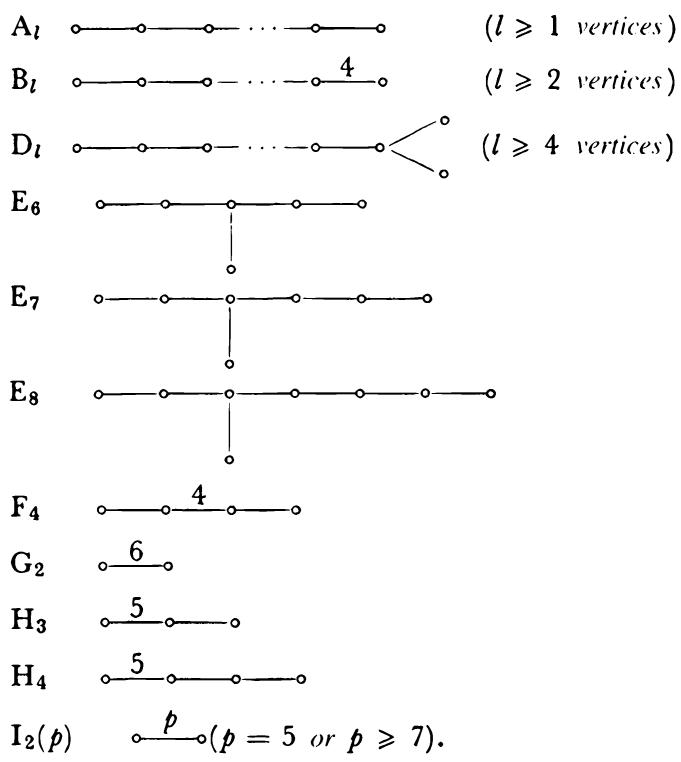
\includegraphics[keepaspectratio]{images/part002_677d99d4.jpg}}

No two of these graphs are isomorphic.

Indeed, let \(\mathrm{W} = (m_{ij})\) be the Coxeter matrix of (W,S), and let \(l = \operatorname{Card}(S)\) . If one of the \(m_{ij}\) is \(\geqslant 6\) , then l = 2 (Lemma 4) and the Coxeter graph of (W,S) is of type \(G_{2}\) or \(I_{2}(p)\) with \(p \geqslant 7\) . Assume now that all the \(m_{ij} \leqslant 5\) .

\begin{enumerate}
\def\labelenumi{\alph{enumi})}
\item
  If the \(m_{ij}\) are not all equal to 3, the graph X of (W.S) is a chain and exactly one of the \(m_{ij}\) is equal to 4 or 5 (Lemma 7). If one of the \(m_{ij}\) is equal to 5, Lemma 9 shows that we have one of the types \(H_{3}\) , \(H_{4}\) or \(I_{2}(5)\) . If one of the \(m_{ij}\) is equal to 4, Lemma 9 shows that we have one of the types \(B_{l}\) or \(F_{4}\) .
\item
  Assume now that all the \(m_{ij}\) are equal to 3. If X is a chain, the Coxeter graph is of type \(A_{l}\) . If not, Lemma 10 shows that it is of type \(E_{6}\) , \(E_{7}\) , \(E_{8}\) or \(D_{l}\) .
\end{enumerate}

The fact that no two of the Coxeter graphs listed are isomorphic is clear.

Conversely:

THEOREM 2. The Coxeter groups defined by the Coxeter graphs \(\mathbf{A}_l, \mathbf{B}_l, \ldots, \mathbf{I}_2(p)\) of Th. 1 are finite.

This is clear for \(I_{2}(p)\) , the corresponding group being the dihedral group of order 2p (Chap. IV, § 1, no. 9). For \(H_{4}\) the corresponding quadratic form

is

\[
\begin{array}{r l} & \xi_ {1} ^ {2} + \xi_ {2} ^ {2} + \xi_ {3} ^ {2} + \xi_ {4} ^ {2} - \xi_ {1} \xi_ {2} - \xi_ {2} \xi_ {3} - 2 (\cos \frac {\pi}{5}) \xi_ {3} \xi_ {4} \\ & = \xi_ {1} ^ {2} + \xi_ {2} ^ {2} + \xi_ {3} ^ {2} + \xi_ {4} ^ {2} - \xi_ {1} \xi_ {2} - \xi_ {2} \xi_ {3} - \frac {1 + \sqrt {5}}{2} \xi_ {3} \xi_ {4} \\ & = (\xi_ {2} - \frac {\xi_ {1} + \xi_ {3}}{2}) ^ {2} + (\xi_ {4} - \frac {1 + \sqrt {5}}{4} \xi_ {3}) ^ {2} + \frac {3}{4} (\xi_ {1} - \frac {1}{3} \xi_ {3}) ^ {2} + \frac {7 - 3 \sqrt {5}}{24} \xi_ {3} ^ {2}. \end{array}
\]

Since \(7 - 3\sqrt{5}\) is \textgreater0, this form is positive non-degenerate, and the corresponding Coxeter group is finite. The same holds for that corresponding to \(H_{3}\) , since it is isomorphic to a subgroup of the preceding (Chap. IV, § 1, no. 8).

For the types \(A_{l}\) , \(B_{l}, \ldots, G_{2}\) , we shall construct, in Nos. 5 to 13, root systems having the corresponding groups as Weyl groups. We shall see that these groups are not only finite, but crystallographic (§ 2, no. 5).

